\chapter{Existující přístupy}

Dynamicky vyvažovaná obtížnost se zdá aktuálním tématem a možná v budoucnu zcela nahradí obtížnost statickou. Většina nalezených a citovaných článků byla napsána po roce 2000, velká část z nich vznikla až po roce 2010. Není tedy překvapením, že existující přístupy pro DDA pokrývají velkou část oblastí v AI obecně. Nalezneme zde case-base reasoning, fuzzy logiku, evoluční algoritmy, neuronové sítě, mravenčí kolonie i příklady z teorie her.

Algoritmy můžeme zařadit do kategorií zmíněných v první kapitole. Klasifikaci jsem provedl na základě vědeckých článků, kde danou metodu použili. Ne ve všech případech bylo zařazení metod jednoznačné, a proto tabulka \ref{tab:klasifikacemetod} reflektuje i můj subjektivní názor. Tabulka může na první pohled vypadat podivně, stejný přístup je často označen za explicitní i implicitní nebo statický i dynamický. 

Explicitnost a implicitnost nevychází přímo z použité metody, ale záleží na designérovi, pro kterou z těchto kategorií se rozhodne. Z tohoto důvodu lze zařadit všechny zmíněné metody do implicitní i explicitní kategorie. Nikdy nemusí být hráč obeznámen s použitím DDA. Do explicitní kategorie jsem zařadil pouze evoluční algoritmus, POSM a dynamickou úroveň. Tyto přístupy pracují s hodnotou obtížnosti, která je snadno zobrazitelná uživateli s jejím jasným významem.

\begin{table*}[b]\footnotesize
\vspace*{0mm}
\caption{{\label{tab:klasifikacemetod}} Klasifikace metod do různých tříd. Mnohdy je zařazení nejasné, a proto je tabulka z části tvořena subjektivním pohledem.}
\vspace*{0mm}
\label{shadowtable}
\begin{center}
\begin{tabular}{| l || c | c || c | c || c | c | c |}
\hline
Metoda DDA & explicitní & implicitní & statická & dynamická & NPC & svět & úkoly \\
\hline
\hline
Producent – konzument  & & \checkmark & \checkmark & \checkmark & \checkmark & \checkmark &  \\ \hline
Case-base reasoning  & & \checkmark &  & \checkmark & \checkmark & & \\ \hline
Fuzzy pravidla  & & \checkmark & & \checkmark & \checkmark & & \\ \hline
Evoluční algoritmus & \checkmark & \checkmark & \checkmark & & & \checkmark & \\ \hline
Mravenčí feromony  &  & \checkmark & & \checkmark & & & \checkmark \\ \hline
POSM & \checkmark & \checkmark & \checkmark & \checkmark & \checkmark & \checkmark & \checkmark \\ \hline
Dynamická úroveň  & \checkmark & \checkmark & & \checkmark & \checkmark & & \\ \hline
MCTS  & & \checkmark & & \checkmark & \checkmark & & \\ \hline
\end{tabular}
\end{center}
\end{table*}

Mimo evoluční algoritmus lze všechny metody zařadit mezi online algoritmy. Přístup producent-konzument je i offline algoritmem. Byl využit u střílečky z pohledu první osoby. Staticky je zde přizpůsobován svět, když do něho hráč vstoupí. Naopak dynamicky se upravuje přesnost a účinnost střelby nepřátel během boje. POSM patří k velice obecným přístupům. Vyžaduje na designérovi návrh konečného množství obtížností a algoritmus z nich posléze vybírá nejvhodnější obtížnost v danou dobu. Z tohoto důvodu je zcela na návrháři, jestli obtížnost bude měněna jen před začátkem hry na základě předchozích her, nebo bude měněna i v průběhu.

Poslední trojice kategorií představuje, čím je dána obtížnost hry. Ve většině případů upravovali umělou inteligenci protihráčů. Jak už bylo zmíněno, producent-konzument upravoval kromě NPC i svět, u POSM je volba obtížnosti na návrháři. Evoluční algoritmus byl využit pro generování úrovní do logické hry. POMDP spolu se simulací mravenců byly využity u vážných her. V obou případech se měnil druh úkolu dle jeho obtížnosti.

\section{Producent – konzument}

V mnohých hrách můžeme pozorovat vztah producent – konzument mezi světem a hráčem. Jestliže hráč získá ze světa moc prostředků, hra přestává být výzvou a naopak. Má-li hráč málo prostředku (např. munice, zdraví), může být frustrován kvůli vysoké obtížnosti.
Robin Hunicke popsala systém The Hamlet\cite{20Hun} integrovaný do Half-Life SDK\cite{hlsdk}, který vyvažuje obtížnost hry právě pomocí výměny zdrojů mezi světem a hráčem. Half-Life patří mezi klasické zástupce first-person shooter (FPS, „střílečky“).

\subsection{Použitá metrika}

Hunicke používá metriku pravděpodobnost smrti hráče. Ze série měření určí pravděpodobnostní distribuci poškození udělené hráči protivníkem během boje. Předpokládá Gaussovskou distribuci :

\begin{equation}
	   p(x)=\frac{1}{\sigma\sqrt{2\pi}}\mathrm{e}^{\frac{-(x-\mu)^2/2}{\sigma^2}}
\end{equation}

Pomocí určitého integrálu F(d) můžeme spočítat pravděpodobnost utrpění poškození menší, nebo rovnu d, kterou lze využít pro určení pravděpodobnosti přežití, jestliže má hráč aktuální zdraví rovné hodnotě d.

\begin{equation}
	   F(x) = \int_d^\infty p(x)\,\mathrm{d}x
\end{equation}

Dosazením za p(x) získáváme rovnici \ref{eq:integraldamage}.

\begin{equation} \label{eq:integraldamage}
	   F(x) = \frac{1}{\sigma\sqrt{2\pi}}\int_d^\infty \mathrm{e}^{\frac{-(x-\mu)^2/2}{\sigma^2}}\,\mathrm{d}x
\end{equation}

Tento integrál lze aproximovat funkcí erf z knihovny C++. V následujícím vzorci h odpovídá aktuálnímu zdraví hráče, $\mu, \sigma$ pro střední hodnotu a standardní odchylku poškození od aktuálního oponenta v nějakém čase t v budoucnu.

\begin{equation}
	   F(d_t) = 1-\frac{1}{2}(1+erf(\frac{h-\mu t}{\sigma\sqrt{2t}}))
\end{equation}

Během souboje se zaznamenává poškození d, které každý z protivníků udělí hráči. Na základě těchto hodnot a vzorců výše lze přibližně spočítat pravděpodobnost smrti hráče.

\subsection{Vyvažující strategie}

Systém Hamlet mění obtížnost na základě poptávky a nabídky. Na straně nabídky může systém zasáhnout umisťováním předmětů v herním prostředí (lékárničky, munice, zbraně). Dále může přizpůsobovat účinnost a přesnost hráčových zbraních, projev brnění apod.

Na straně poptávky manipulovat s nepřáteli (změnou jejich třídy, množství, počtu jejich životů, určením místa jejich objevení se na mapě). Stejně jako u hráče lze přizpůsobit sílu a přesnost jejich zbraní.

Autoři se snaží držet hráče v tzv. „komfortní zóně“, kdy se hráč cítí relativně v bezpečí. Jestliže se v průběhu boje zvedne pravděpodobnost úmrtí nad 40\%, Hamlet začne zasahovat do hry výše uvedenými způsoby.

Cílem této politiky je udržet zdraví hráče na střední hodnotě 60 se standardní odchylkou 15 bodů. Hamlet je navržen tak, aby pomáhal hráčům, kteří mají problémy, ale na druhou stranu, aby je neprotahoval za každou cenu skrz herní úrovně.

\subsection{Výsledky}

DDA systém byl ověřen při experimentu, kterého se účastnilo 20 osob různé úrovně. Každá osoba absolvovala dvě hry v délce alespoň 15 minut. V jedné hře bylo zapnuté dynamické vyvažování obtížnosti, v druhé nikoli.

Zaznamenával se počet smrtí během prvních 15 minut hry. Nakonec každý z účastníku odpověděl, která z her ho bavila více.

Střední hodnota a směrodatná odchylka počtu smrtí u vyvažované hry byly rovny 4 a 3,0, u nevyvažované 6,4 a 2,1.

U začátečníků se neprojevila souvislost mezi použitím/nepoužítím DDA a pocitem zábavy, pokročilí hráči více upřednostňovali použití DDA.

\section{Case-base reasoning} \label{sec:CBR}

Další možností pro implementaci DDA je Case-base reasoning(CBR). CBR metoda používá databázi stavů s ohodnocením jednotlivých hráčů v daném stavu a se strategiemi, které hráči v tu chvíli používali. Při rozhodování hráč vždy nahlédne do databáze, vybere několik stavů podobných současnému a vybere z nich ten nejvhodnější. Pokud se snažíme o co nejlepšího hráče, vybere se z podobných stavů stav, kde dosahuje hráč nejlepšího výsledku. Při aplikaci DDA bude nejvhodnějším stavem stav, kdy jsou síly vyrovnané.

Tento přístup byl využit u strategické hry Spring. \cite{21cbr} Proces celé adaptivní AI znázorňuje diagram Obr. \ref{fig:ch3cbrspring}.
Začne se sběrem dat (game observation). Proběhne simulace stovek her s různými hráči a vždy se v průběhu hry v určitých intervalech zaznamená zjednodušený popis stavu hry, použité strategie všech hráčů. 

Následuje offline zpracování (A. Offline processing), které může být časově náročné. Jednotlivé stavy se ohodnotí číslem (Game indexing). Dle předem známé heuristiky se určí, který z hráčů vede a „o kolik“. Kvůli velké paměťové náročnosti a posléze náročnosti vyhledávání v databázi se data komprimují pomocí shlukování (Clustering of observations). Situace hry navzájem si podobné se nahradí situací jednou.
 
\begin{figure}
  \centering
  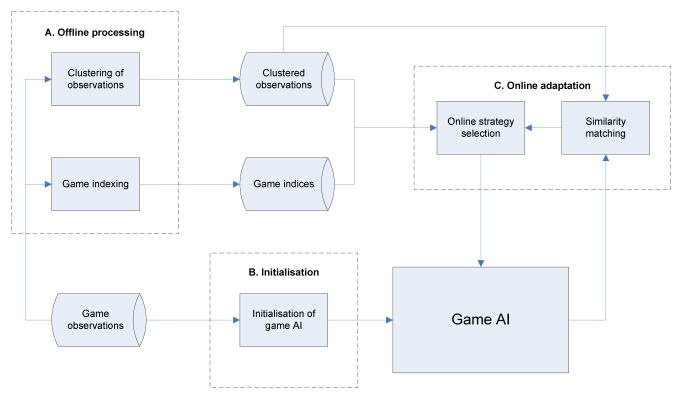
\includegraphics[width=0.8\textwidth]{ch3cbrspring}
	\caption{Proces adaptivní AI založené na CBR \cite{21cbr}}
	\label{fig:ch3cbrspring}
\end{figure}

Při inicializaci (B. Initialisation) se nastaví první strategie AI, která se ukázala nejlepší v daném scénáři. Poslední části schématu je online adaptace (C. Online adaptation), která nesmí být náročná na výpočetní výkon, jelikož se provádí v reálném čase. V určitých intervalech během hry se změní strategie hráče (Online strategy selection) na strategii, která se ukázala nejvhodnější v podobné situaci(Similarity matching).

\subsection{Sběr a úprava dat}

Při sběru dat pro adaptivní AI ve hře Spring získali 448 567 pozorování z celkem 975 her na třech různých herních mapách. Výsledná data zabírala 1192 MB nekomprimovaně. Spouštěli se vždy hry s dvěma protihráči. Pokaždé inicializováni různými strategiemi. V tomto kontextu se strategií míní vektor celkem 27 parametrů představující důraz na různé strategické chování na vysoké úrovni. Např. parametr aircraft\_rate ovlivňuje, jak moc často by měl hráč vytvářet vzdušné jednotky. Jakým způsobem se toho dosáhne už nesouvisí s těmito parametry. Dále je nutné popsat a uložit popis dané situace, jež se později použije pro vyhledávání podobných pozorování. Pozorování je popsáno 6 parametry. Fáze hry, síla materiálu, bezpečí velitele, ovládané území, ekonomická síla a počet vojenských jednotek.

\subsection{Ohodnocení her}

Každé z pozorováních se ohodnotí pomocí fitness funkce. Získané číslo určuje, kdo v dané chvíli vítězí. Fitness hodnota blížící se nule značí vyrovnané síly obou soupeřů. Vypočítá se např. z fáze hry, množství surovin a jednotek jednotlivých hráčů.

\subsection{Shlukování pozorování}

Shlukování je velice časově náročné, a proto se provádí offline. Cílem je nahradit více pozorováních jedním reprezentantem, který může být jedním pozorováním z původních dat, nebo pozorování vzniklé zprůměrováním podobných dat. Záleží na zvoleném algoritmu. Zde postačil dobře známý a jednoduchý algoritmus k-means\cite{kmeans}.

\subsection{Inicializace hry}

V této fázi procesu se určí první strategie dynamické AI. Nejdříve se určí strategie, kterou využívá soupeř. Z ní se udělá abstrakce, jednotlivé hodnoty 27 proměnných se nahradí hodnotou z výčtu „málo“, „středně“, „hodně“.  Poté se naleznou v databázi pozorování s hráči podobnými soupeři a vybere se inicializační strategie, která si vedla nejlépe proti takovému hráči. Z tohoto důvodu nikdy není vybrána neefektivní strategie jako první.

\subsection{Online adaptace}

V průběhu hry se čas od času spustí adaptace herní strategie dle aktuálního stavu hry. Tato adaptace se skládá ze dvou částí, z porovnávání stavů a výběru strategie.

Podobnost dvou pozorování je rovna váženě sumě podobnosti šestice parametrů v jednotlivých pozorováních.

\begin{equation}
	   podobnost(poz1,poz2)=((1+f)*(0,5*u)) + mp + sc + cp + ep
\end{equation}

\begin{eqnarray*}
f &= &rozdilFazeHry(poz1,poz2) \\
u &= &rozdilPoctuJednotek(poz1,poz2) \\
mp &= &rozdilMaterialniSily(poz1,poz2) \\
sc &= &rozdilBezpecnostiVelitele(poz1,poz2) \\
cp &= &rozdilObsazenychPozic(poz1,poz2) \\
ep &= &rozdilEkonomickeSily(poz1,poz2)
\end{eqnarray*}

Samotná selekce nejvhodnější strategie se skládá ze tří kroků. Nejdříve se z databáze shluků vybere N nejbližších sousedů k aktuálnímu stavu hry dle výše uvedeného vzorce. Posléze se vybere menší podmnožina M stavů na základě herního indexu(fitness) dle zvoleného kritéria.

Zde se může projevit kombinace statické volby obtížnosti s dynamickou. Hráč si může před začátkem hry z volit jednu z pevně daných obtížností, např. lehká, normální, těžká. Vybere-li si běžnou obtížnost, bude algoritmus vybírat M stavů, jež mají fitness nejblíže k 0, která značí vyrovnané šance obou hráčů na výhru. Naopak hraje-li těžkou hru, algoritmus může vybírat pozorování s fitness odpovídající větší šance na výhru soupeřem.

Zbývá vybrat jedinou novou cílovou strategii. Z M stavů se vybere takový stav, kde strategie soupeře nejvíce odpovídá aktuální strategii soupeře v současné hře.

\subsection{Provedené experimenty}

Autoři článku provedli dva typy experimentů. V prvním se adaptivní hráč snažil chovat co nejlépe, jeho cílem bylo porazit nepřítele. V druhém případě měl adaptivní hráč za úkol udržovat co nejdéle vyrovnaný stav hry. Oponentem adaptivnímu hráči byl v jednom případě umělý hráč z originální hry(AAI) a v druhém případě hráč s náhodně nagenerovanou strategií. Pro srovnání pustili stejné experimenty s adaptivním hráčem, který měl vypnutou adaptivitu, jeho strategie se v průběhu hry neměnila.

Proti AAI hráč vyhrál ve 39\% her, když neměl zapnutou adaptivitu, a ve 77\% se zapnutou adaptivitou. Proti náhodnému soupeři vyhrál bez adaptivity v 47\% případů, s adaptivitou v 64\% her.

Při druhém experimentu adaptivní hráč udržoval vyrovnaný stav hry průměrně 37 minut proti AAI a 36 minut proti náhodnému protihráči. Bez DDA byl vyrovnaný stav 27 a 28 minut proti AAI a náhodnému hráči.

Výsledky obou experimentů byly pozitivní. DDA v tomto případě mělo smysl.

\section{Fuzzy pravidla} \label{sec:fuzzy}

Tento princip využívá fuzzy logiku. Fuzzy logika se od klasické logiky liší především funkcí příslušnosti. U ostrých množin prvek buď do množiny patří, nebo nepatří. Ve fuzzy logice lze popsat situace, kdy prvek do množiny patří pouze z části.

Mějme rozhodovací pravidlo ve strategické hře : Pokud je blízko soupeřova armáda a je velká, začni rekrutovat hodně vojáků. Pojmy blízko, velká, hodně jsou neurčité. Bez fuzzy logiky bychom pravidlo mohli zapsat ve tvaru Pokud je soupeřova armáda vzdálená do 100m a má sílu větší než 1000 jednotek, začni rekrutovat 100 vojáků. Nedostatkem tohoto ostrého pravidla je, že pokud bude armáda mít sílu 999 jednotek, pravidlo se neaplikuje. Tento nedostatek lze eliminovat pomocí fuzzy pravidel. Fuzzy pravidla nemají ostré hranice, kdy se aplikují a kdy naopak ne. V případě, že se některé podmínky nesplní jen těsně, pravidlo se stále provede, ale s menším efektem. V daném příkladu by to mohlo znamenat pouze vytvoření menšího počtu vojáků.

Základní myšlenka DDA založené na fuzzy pravidlech je jednoduchá. Mějme databázi fuzzy pravidel, kde každé z fuzzy pravidel může být aktivní, nebo vypnuté. Jestliže se hra jeví příliš těžká, vybere se některé z pravidel, a to se vypne. Naopak v případě, kdy se hra jeví příliš jednoduchá, jedno pravidlo se znovu aktivuje. Tímto způsobem se dynamicky upravuje umělá inteligence hráčů.

\subsection{Dead-end}

Autoři přístupu zvolili pro jeho testování hru jednoduchou hru Dead-end.\cite{25deadend} Hráč je obklopen třemi stěnami a na čtvrté straně je východ. Jeho cílem uniknout tímto východem. Jeho snažení brání nepřátelské figury, které se naopak snaží hráče chytnout. Hráč má několik životů. Jestliže dojde ke kolizi hráče s nepřátelským duchem, jeden život ztratí. Ztratí-li všechny životy, hráč prohrává. Ve hře je navíc nastaven časový limit. Vyprší-li tento limit, hráč také prohrává. Naopak dostane-li se ven s alespoň jedním životem, vyhrává. Všechny postavičky se mohou pohybovat osmi směry.

Duchy lze rozdělit do dvou rolí. Duch nejníže vzhledem k souřadnici y tvoří předvoj a jistým způsobem ovládá ostatní duchy, obránce.

\begin{figure}
  \centering
  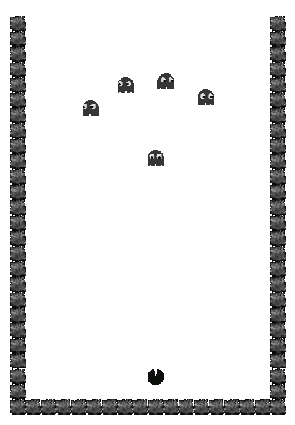
\includegraphics{ch3deadend}
	\caption{Screenshot ze hry Dead-End. \cite{25deadend} }
	\label{ch3deadend}
\end{figure}

\subsection{Fuzzy pravidla}

Duši se rozhodují na základě 5 vstupních fuzzy proměnných, jedné ostré proměnné a pěti výstupních proměnných.
Vstupními proměnnými pro pravidla předvoje jsou vzdálenost k hráči, vzdálenost k východu na ose y,  vzdálenost k hráči na ose x a binární proměnná, jestli duch už prošel kolem předvoje. Výstupními proměnnými jsou proměnné pro akce, které může duch provést – chytej hráče, nebo ustupuj od hráče.

Vstupní fuzzy proměnné pro obránce jsou vzdálenost k hráči, vzdálenost k předvoji, vzdálenost k nejbližšími jinému obránci na ose x a stejná binární proměnná značící, jestli byl už duch obejit.

Možné akce obránců jsou – chytej hráče, přibliž se k předvoji, oddal se od předvoje, oddal se od nejbližšího jiného obránce.
Příkladem fuzzy pravidla pro předvoj z kompletní tabulky 40 pravidel z \cite{25deadend} :
Pokud je hráč blízko předvoje a je blízko východu a hráč ještě neprošel kolem předvoje, pak chytej hráče velmi. Viz první pravidlo z následujícího obrázku Obr. \ref{fig-ch3fuzzytable}.

\begin{figure}
  \centering
  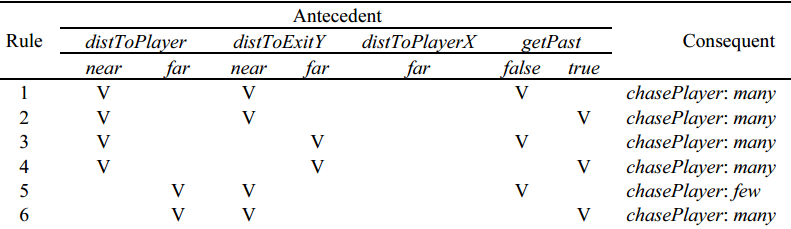
\includegraphics[width=0.75\textwidth]{ch3fuzzytable}
	\caption{Část fuzzy pravidel pro předvoj. \cite{25deadend} }
	\label{fig-ch3fuzzytable}
\end{figure}

Uvedené příklady fuzzy proměnných a pravidel by měli pro základní představu postačovat. Kompletní seznam fuzzy pravidel a detailnější popis jednotlivých proměnných včetně grafů funkce příslušnosti lze najít v již zmiňovaném zdroji \cite{25deadend}.

\subsection{Adaptivní změna počtu pravidel}

Jestliže se soupeř řídí všemi 40 pravidly, chová se velmi inteligentně. Hráč si na začátku hry může vybrat statickou část obtížnosti. Může ovlivnit požadovaný win-rate. Pokud tak neučiní, nastaví se win-rate na hodnotu 50\%. Každá hra trvá maximálně 20 vteřin. V případě, že hráč vyhraje a aktuální poměr vítězství/proher  je větší než cílená hodnota, hra se musí ztížit aktivováním momentálně vypnutého pravidla.

Naopak v případě, že hráč prohraje a aktuální hodnota win-rate je menší než cílená, hra je příliš těžká, zjednodušení proběhne deaktivací jednoho z pravidel.

Pokaždé, když se duch rozhodne dle jednoho z pravidel, zaznamená se to. Výsledný příspěvek se u pravidel obránců vydělí 4, jelikož jsou ve hře 4 obránci a jen jeden předvoj.

Pokud má dojít k deaktivaci pravidla, deaktivuje se pravidlo, které bylo využito nejméně krát, ale alespoň jednou. Kdyby se vyřadilo pravidlo, které se nevyužilo, hráč by nemusel vůbec změnu obtížnosti v příští hře poznat, jelikož by se mohli duchová chovat zcela stejně. Pokud by se deaktivovalo pravidlo, které používal soupeř nejvíce, mohla by být změna obtížnosti příliš drastická a mohlo by to vést k neočekávaným výsledkům.

Reaktivace pravidla je o něco složitější proces. Nejdříve se všechna pravidla rozdělí do skupin dle jejich konsekventů. Příspěvek celé skupiny pravidel je roven sumě příspěvků jednotlivých pravidel ve skupině. 

Poté se spočte suma vstupních příslušností hodnot pro každé z pravidel deaktivovaných dříve. Nakonec se zaktivuje pravidlo s největší sumou vstupních příslušností. Jestliže existují dvě pravidla se stejnou hodnotou sumy, zvolí se pravidlo jehož skupina má nejnižší příspěvek.

\subsection{Výsledky}

Na závěr připojuji jeden z grafů ukazující adaptivnost AI k třem různým hráčům s požadovanou hodnotou win-rate 75\% Obr. \ref{fig-ch3fuzzywinrate}. Ke srovnání na cílovou hodnotu došlo kolem 25. hry. Znamená to, že stačilo přibližně 25 her k upravení množiny pravidel, aby hráč vyhrával v 75\% případů, což byla cílová hodnota win-rate.

\begin{figure}
  \centering
  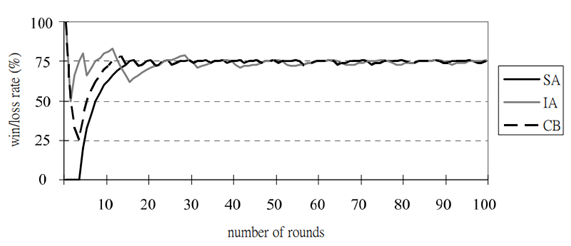
\includegraphics[width=0.75\textwidth]{ch3fuzzywinrate}
	\caption{Přibližování se k požadovanému win-rate 75\% během 100 kol proti třem různým hráčům. \cite{25deadend} }
	\label{fig-ch3fuzzywinrate}
\end{figure}

\section{Evoluční algoritmus} \label{sec:evol}

K zástupcům statické DDA patří evoluční algoritmy (EA). Evoluční algoritmy zpravidla vyžadují velký výpočetní výkon, a proto nejsou vhodné pro realtime použití. Využitím EA pro DDA se zabývají např. články Automatic Generation of Game Elements via Evolution\cite{17Evol} a Making Racing Fun Through Player Modeling
and Track Evolution\cite{EvolTrack}. V prvním ze zmíněných článků využili EA pro generování různě obtížných úrovní logických her, naopak v druhém generovali závodní trať složenou z různých úseků.

Evoluční algoritmy jsou inspirovány evolucí známou s přírody, kde se nejsilnější jedinci dále množí a naopak nejslabší hynou, což vede ke stále silnějším generacím. Umělá evoluce je iterativní proces, který neustále opakuje několik kroků. Vždy se vybere několik jedinců, kteří se zkříží a vzniknou noví potomci. Následně může proběhnout mutace, která může zanést do populace gen, který se v ní nevyskytoval. Noví potomci poté nahradí nejslabší a celý proces se opakuje.

Definice jedince, způsobu výběru nejsilnějších, křížení a mutace je vždy závislá na problému, kde je evoluční algoritmus použit. Konkrétní případy budou popsány zvlášť u každého problému v podsekcích této sekce.

\subsection{Generování bludišť}

V práci \cite{17Evol} byl evoluční algoritmus použit pro generování logických hádanek s předem zadanou obtížností.

Testovacími hrami dva typy bludišť. V obou hrách byl stejný cíl, nalézt cestu mezi dvěma body. Obě bludiště dále sdílely hrací plán složený ze čtverců a nepřímo znázorněné překážky. Obtížnost hry je dána minimálním počtem kroků nutných k průchodu bludištěm. Neplatí zde zcela přímá úměra, obecně neplatí, že čím větší minimální počet kroků k dosažení cíle, tím je hra těžší. V případě, že bychom minimální počet kroků zcela maximalizovali, získáme bludiště, kde na začátku každý z tahů vede blíže k výhře. 

Hráč nemá dostatek možných tahů na výběr, a tedy je bludiště jednodušší než kdyby minimální počet kroků byl menší, ale naopak počet možných tahů by se zvýšil a ne všechny tahy by vedly blíže k cíli. Tuto hypotézu podporují informace získané při automatickém průchodu bludišť nutného pro ohodnocení obtížnosti hry. Algoritmus řešící bludiště se střední hodnotou minimálního počtu kroků pro daný typ bludiště běžel kratší dobu než pro bludiště s hodnotami blízkými minimu a maximu minimálnímu počtu kroků.

V první hře hráč pohybuje šachovou figurkou dle jejích platných tahů. Dále se na hracím plánu vyskytují nepřátelské šachové figury, které se nepohybují. Tyto figury ohrožují některá hrací pole. Jestliže hráč vkročí svou figurou na ohrožené hrací pole, prohrává. Jeho úkolem je figurku navést z její počáteční pozice do cílové a přitom nevkročit na žádné z ohrožovaných polí. Hráč nemá přímo označena ohrožená pole, musí využít své představivosti. Před generováním bludišť byly vždy pevně nastaveny druhy figur na hrací ploše, figura hráče a jeho startovní a cílová pozice. Cílem genetického algoritmu bylo rozmístit nepřátelské figury. Příklad jednoho bludiště na obr. \ref{fig-ch3evolchess}.

\begin{figure}
  \centering
  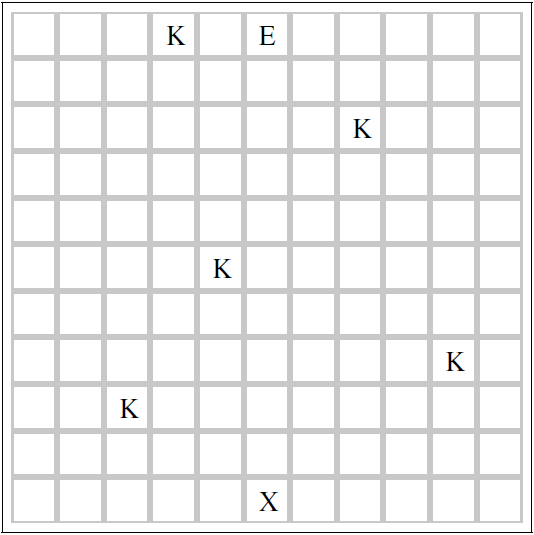
\includegraphics[width=0.3\textwidth]{ch3evolchess}
	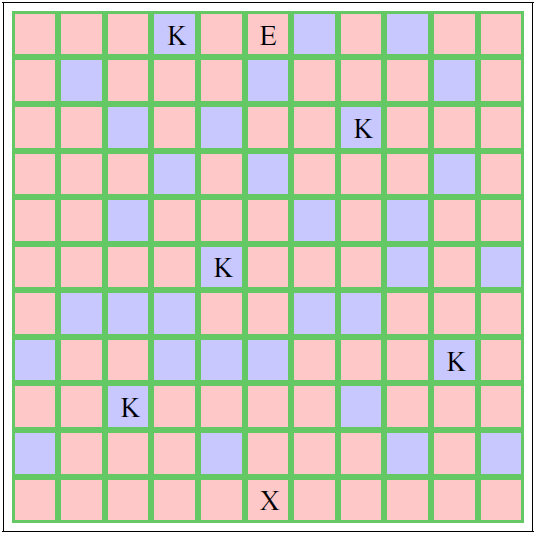
\includegraphics[width=0.3\textwidth]{ch3evolchess2}
	\caption{Příklad jednoho vygenerovaného bludiště se 6 jezdci a hráčem ovládajího věž. Vstup do bludiště je označen E, výstup X. Vlevo z pohledu hráče, vpravo znázorněné ohrožované pozice. \cite{17Evol} }
	\label{fig-ch3evolchess}
\end{figure}

Gen byl složen z pozic figur. Pro stejný druh figur nezáleželo na jejich pořadí. Bylo použito uniformní křížení. První ze dvou potomků má stejnou šanci pro získání pozice každé z figur jak od matky, tak i otce. Zbytek získá druhý potomek. Jestliže se po křížení nacházely u jednoho z potomků dvě figury na jedné pozici, potomci se zahodili, křížení se opakovalo. Při mutaci byla pozice jedné z figur náhodně přegenerována na ještě neobsazené pozice.

Druhou hrou bylo pestrobarevné bludiště. Každý čtverec bludiště má přidělenou jednu barvu z předem dané uspořádané množiny barev. Hráč se může mezi dvěma čtverci pohnout pouze v případě, kdy přechází mezi čtverci s barvami stejnými, nebo sousedními v rámci uspořádání. Opět při nepovoleném tahu hráč prohrává.

Gen je zde tvořen celým bludištěm uspořádaným po řádcích do jednoho řetězce o délce počtu čtverců bludiště. Bylo použito dvoubodové křížení a při mutaci se náhodně vybral jeden čtverec a vygenerovala se mu nová barva dle uniformního rozdělení pravděpodobnosti.

U obou her EA pracoval se stálou (steady-state) populací a selekce rodičů probíhala metodou turnaje. Vždy bylo vybráno náhodně 7 jedinců z celé populace, dva nejlepší z nich byli vybráni pro křížení a noví jedinci nahradili nejhorší dvojici vybranou pro turnaj.

Byly použity dvě fitness funkce. První maximalizovala minimální počet kroků k vyřešení bludiště. Druhá měla parametr - cílovou hodnotu minimálního počtu kroků - a tato fitness funkce minimalizovala rozdíl skutečného minimálního počtu kroků od požadovaného. Pro výpočet této hodnoty autoři článku využili metodu dynamického programování.

V proběhnutých experimentech algoritmus dokázal vyvinout bludiště s předem zadanou obtížností, a tedy splnil svůj účel.

\subsection{Generování tratě}

Cílem práce \cite{EvolTrack} bylo procedurální generování co nejzábavnějších tratí pro závodní hry. Autoři článku za základě vlastních zkušeností a zkušeností dotazovaných hráčů definovali, jaká by měla být závodní hra, aby byla zábavná:

\begin{itemize}
	\item Hráči rádi jezdí co největší rychlostí. Trať by měla umožňovat dosažení maximální rychlosti aut.
	\item Naopak pouze jízda po dlouhých rovných úsecích není zábavná. Trať by měla být určitou výzvou pro hráče.
	\item Lidé mají rádi různorodé výzvy. Jednotlivé tratě by měly poskytovat dostatečnou variabilitu výzev.
	\item Ježdění ve smyku a skoky autem se zdají být jednou ze základních složek zábavy závodních her.
\end{itemize}

Pro zjednodušení se generovaná trať skládala s předem daného počtu stejně dlouhých úseků.\footnote{Délka úseku dána délkou střední čáry.} Úsek mohl být rovný, nebo zatáčkou vlevo, či vpravo. Každá ze zatáček měla na výběr mezi 3 ostrostmi zatáčky. Dále gen obsahoval jednu ze tří šířek konce úseku. Začátek úseku vždy musel odpovídat šířkou konci úseku předchozího. Poslední variabilitou bylo umístění překážky na jeden z krajů úseku, nebo doprostřed. Dalším zjednodušením bylo vypuštění podmínky na kruhové trati. Trať byla pouze virtuálně kruhová - na jejím konci se hráč teleportoval na začátek se stejnou rychlostí a směrem jízdy. Křížení genů nebylo využito. Mutace změnila náhodně jeden z úseků na nový dle uniformní pravděpodobnosti.

\begin{figure}
  \centering
  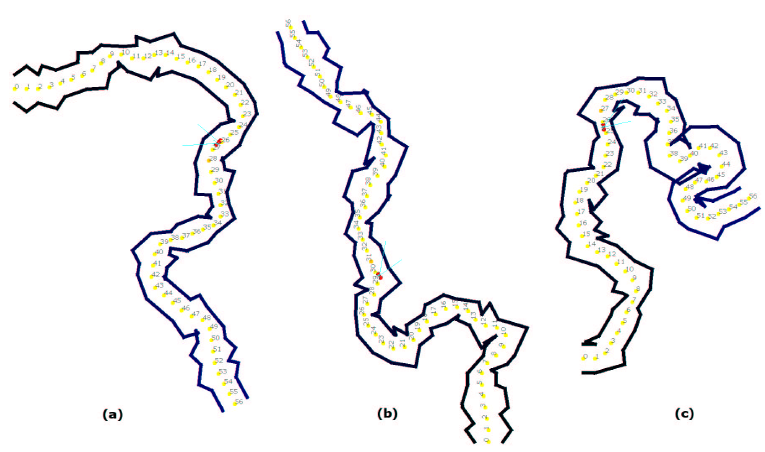
\includegraphics[width=0.75\textwidth]{ch3evoltrack}
	\caption{Příklad tří vygenerovaných tratí. První generována pro špatného hráče, druhá a třetí pro dobrého. Při generaci třetí tratě byla použita pouze jedna z fitness funkcí. \cite{EvolTrack} }
	\label{fig-ch3evoltrack}
\end{figure}

Metodou selekce byl kaskádový elitismus. Nejdříve se nagenerovalo 100 jedinců. Dle první fitness funkce se vybralo 50 nejlepších jedinců, kteří postoupili do druhého kola. V druhém kole se použila jiná, druhá fitness funkce, která vyřadila dalších 20 nejhorších jedinců. Ze zbylých 30 skončilo 15 nejlepších dle poslední třetí fitness funkce. První fitness funkci minimalizovala rozdíl cílené(předem dané parametrem) a skutečné hodnotě průměrné rychlosti na trati. Druhá fitness funkce maximalizovala maximální dosaženou rychlost na trati. Cílem bylo, aby trať obsahovala alespoň nějakou posloupnost rovných úseků. Poslední fitness funkce se zaměřila na měření množství výzev na trati. Vycházela z variance rychlosti na trati a počtu ujetých kol za danou dobu. 

Každá z vygenerovaných tratí byla vyzkoušena virtuálním hráčem nahrazující lidského hráče založeného na neuronových sítí. Vstupem do sítě byla aktuální rychlost, směr k dalšími checkpointu a 6 senzorů sledujících překážky.

Během experimentů byly mimo jiné vytvořeny tři tratě zobrazené na obr. \ref{fig-ch3evoltrack}. Dle nastaveného parametru měla být první trať jednoduché, další dvě složitější. Závěrem lze říci, že se povedlo vygenerovat tratě s cílenou obtížností, kde první je bez ostrých zatáček, ale naopak v dalších dvou se ostré zatáčky objevují.

\subsection{Mravenčí feromony} \label{sec:ants}

Optimalizace pomocí simulace umělých mravenčích kolonií patří mezi známé přístupy inspirované přírodou. Princip optimalizace mravenčími koloniemi je následující :

\begin{enumerate}
	\item Daný problém se vhodně modeluje jako graf skládající se z uzlů a hran mezi nimi
	\item Umělí mravenci se pohybují po hranách a zanechávají na nich feromon. Čím lépe si vedou, tím více feromonu zanechají.
	\item Mravenci se na každém uzlu rozhodují, kterou další hranou se vydají. S větší pravděpodobností zvolí hrany, na kterých je více zanechaného feromonu.
	\item Časem feromon vyprchává, je třeba obnovovat.
	\item Optimalizace končí, jestliže se ustálí cesty v grafu. 
\end{enumerate}

Tímto algoritmem se inspirovali vývojáři jedné ze serious games určené pro rehabilitaci částečně ochrnutých končetin lidí, jež utrpěli mozkovou mrtvici\cite{26poststroke}.

Cílem práce bylo vytvořit hru, která budu procvičovat znovu ovládnutí pohybu ruky. DDA mělo za úkol adaptivně měnit obtížnost hry a přizpůsobovat se individuálním potřebám pacientů. 

Výsledkem je jednoduchá hra odehrávající se na desce o rozměrech přibližně 1,5m na 1,5m rozdělená do buněk menší velikosti. Hra vždy označí některou z buněk za cílovou a pacient se jí má pokusit dosáhnout pomocí své ruky. Algoritmus mravenčích feromonů zde byl použit pro určení, které buňky jsou pro pacienta už snadno dosažitelné, a které ne.

\subsubsection{Hráčův profil}

Schopnosti pacienta jsou zaznamenávány do tabulky Zóna schopnosti(ability zone). Zóna schopnosti je matice o velikosti m x n. Každá z buněk má přiřazeno reálné číslo reprezentující snadnost dosažení dané buňky. Cílem je vytvořit model obrazu schopností pacienta.
Tato definice pouze popisuje strukturu a zamýšlenou funkci zóny schopnosti, ale již nezmiňuje, jak takovou strukturu vytvořit. Existuje více různých cest.

Jednou z možností je uložit do každé buňky statistickou úspěšnost dosažení buňky pacientem, jestliže to dostal za úkol. Jinou možností jsou biologicky inspirovaní umělí mravenci.

Pacientova ruka představuje mravence, který se pohybuje po mřížce. Na místech, která navštíví, zanechá feromon. Feromon zanechá i na okolních buňkách, ale o něco méně. Čím více feromonu je na buňce zanecháno, tím je pro pacienta jednodušší této buňky dosáhnout, a proto je vhodnější cílit pacientovu ruku do buněk jiných.

\subsubsection{Zákon propagace}

Nově přidaná úroveň feromonu $level_s(c)$ na buňku $c$ mravencem s pozicí $s$ lze spočítat následovně.


\begin{equation}
	level_s(c)= \begin{cases}
											  A(1-\frac{dist(s, c)}{w}) & dist(s, c) \leq w \\
												0 & jinak
										 \end{cases}
\end{equation}

Ve vzorci konstanta $A$ značí nominální úroveň feromonu, jež se přidává na buňku s pozicí mravence, konstanta w značí dosah vlivu feromonu do okolních buněk. Funkce dist vrací vzdálenost mezi dvěma pozicemi předanými argumenty.

\subsubsection{Zákon vyprchávání}

Vyprchávání feromonů je též velice důležité. Zajistí zapomenutí oblastí, které hráč zasáhl pouze náhodou. Jelikož pacientovi pohyby nejsou plně kontrolovatelné, může se stát, že neúmyslně zasáhne některé buňky, které nechce.

Z tohoto důvodu chceme, aby vyprchávali více feromony, jež byly zasáhnuty náhodou. S vědomostí, které buňky zóny schopností pacient zasáhl pohybem po cestě p můžeme upravit množství feromonů na nich.

\begin{equation}
	F_{t+1} = F_t\frac{1}{vrcholyRychlosti(p)}
\end{equation}

Čím více vrcholů v grafu rychlosti na dané cestě, tím více byly pohyby trhané a tedy méně koordinované.

\subsubsection{Matice interakce}

Matice interakce je maticí m x n binárních hodnot. Jednička značí možnost vygenerovat cíl hry z odpovídající buňky, 0 naopak. V případě, že je náročnost hry odpovídající aktuálním schopnostem pacienta, matice interakce se nemění a generují se z ní nové cíle k dosažení rukou. Delší série výher značí, že hra je jednoduchá a hráč může být brzy z nuděn a nemotivován ke hře, k rehabilitaci a naopak delší série proher může způsobovat frustraci se stejným dopadem, koncem rehabilitace a možná i nechutí v ní v budoucnu pokračovat. V takovém případě se matice interakce musí přepočítat.

V obou případech se vypočítá pro každou z buněk jednoduchým vzorečkem gradient.

\begin{equation}
	grad(A_{i,j}) = \sum_{k \in \{i-1, i, i+1\}} \sum_{l \in \{j-1, j, j+1\}} A_{i, j} - A_{k, l}
\end{equation}

V případě příliš obtížné hry bude matice interakce obsahovat 1 na místech kladného gradientu, v opačném případě při příliš lehké hře bude obsahovat 1 v místech záporného gradientu. Příklad na Obr. \ref{fig-ch3feromons}.

\begin{figure}
  \centering
  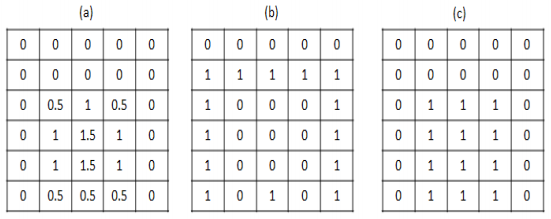
\includegraphics[width=0.75\textwidth]{ch3feromons}
	\caption{(a) Zóna schopností, (b) Interakční matice pro stížení hry, (c) Interakční matice pro zjednodušení hry \cite{26poststroke} }
	\label{fig-ch3feromons}
\end{figure}

První matice (a) obsahuje hodnoty zóny schopností po jednoduchém pohybu „zdola nahoru“ do buňky 3, 3. V matice (b) jsou jedničky na pozicích záporného gradientu dle výše uvedeného vzorce. V matici (c) jsou naopak jedničky na pozicích kladného gradientu. Z matic lze snadno vyčíst ztížení hry u matice (b) a zjednodušení u matice (c).

\subsection{Provedené experimenty}

Autoři přístupu ho otestovali na skupině 10 lidí. Každý dostal nejdříve za úkol si představit, že drží v ruce gumu, a měl touto virtuální gumou vymazat co největší plochu. Následně každému z účastníků experimentu byly generovány pozice na desce, kterých měl účastník svou rukou dosáhnout. Cílem bylo dosáhnout co největšímu počtu pozic během dvou minut. V prvním případě se pozice generovali zcela náhodně, v druhém pomocí představeného DDA principu.

Po skončení experimentů měli účastníci odpovědět, jakou pociťovali obtížnost, frustraci a únavu během obou polovin experimentu.

Výsledky ukázaly, že v případě použití DDA účastníci dosáhli v průměru o 4,3 pozic více než při náhodném generování pozic. Dle subjektivního pocitu účastníci nepociťovali rozdíl v obtížnosti, frustraci a únavě v obou polovinách experimentu.

\section{Částečně uspořádaná množina – Mistr}

Partially-Ordered-Set Master (POSM) \cite{22posm1} je obecně použitelným algoritmem pro dynamicky vyvažovanou obtížnost ve hrách. POSM lze využít kdykoli a v jakémkoli herním žánru. Jediným požadavkem na vývojáře je definovat konečné množství nastavení obtížnosti, pro které existuje relace „je těžší než“. Tento předpoklad není nerealistický. Většina her v současnosti obsahuje několik nastavení statické obtížnosti. Cílem DDA je adaptivně přepínat mezi těmito předdefinovanými obtížnostmi.

Oproti jiným přístupům DDA nevyžaduje modelaci chování hráčů. Nepředpokládá jiné znalosti o konkrétní hře. 
Základní princip algoritmu je jednoduchý. Mistr (program) inicializuje obtížnost na prostřední ze všech obtížností dle relace „je těžší než“ $\geq$. Odehraje se část hry. Posléze se určí, jestli mistr zvolil obtížnost správně dle schopností hráče, nebo jestli hra byla příliš těžká, nebo příliš jednoduchá. Na základě této informace upraví obtížnost hry správným směrem.

\subsection{Algoritmus POSM}

Vstupem algoritmu je částečně uspořádaná množina $(K,\geq)$ možných nastavení obtížnosti. Uspořádání je následující : $\forall i,j \in K$ píšeme $i>j$, pokud $i$ je více obtížné než $j$.
Po nastavení obtížnosti se odehraje kus hry a určí se hráčem pozorovaná obtížnost $o_t$.

\begin{itemize}
	\item $o_t=0$, jestliže obtížnost mistr zvolil správně a nemá se měnit
	\item $o_t=+1$, jestliže obtížnost byla příliš jednoduchá
	\item $o_t=-1$, jestliže obtížnost byla příliš těžká
\end{itemize}
	
Posledním vstupem algoritmu je učící konstanta $\beta\in(0,1)$. Čím blíže je konstanta hodnotě 1, tím je učení pomalejší, obtížnost je více statická.

Kroky algoritmu POSM:

\begin{algorithm}
\caption{Partially-Ordered-Set Master}
\label{posm}
\begin{algorithmic}[1]
\State $\forall k \in K : w_1(k) = 1$
\For{$i \gets 1, 2, \dots$}
	 \State $\forall k \in K : A_t(k) = \sum_{x \in K, x \geq k} w_t(x)$
	 \State $\forall k \in K : B_t(k) = \sum_{x \in K, x \leq k} w_t(x)$
	 \State $k_t = \operatorname{arg\,max}_{x \in K} \min({A_t(x), B_t(x))}$
	 \State Pozoruj reálnou obtížnost $o_t\in \{0,+1,-1\}$
	 \If{$o_t = 1$}
	   \State $\forall k \in K : w_{t+1}(k) = 
		                                        \begin{cases}
																						   \beta w_t(k) & k \leq k_t \\
																							 w_t(k) & jinak
																						\end{cases}
						 $
   \EndIf
	 \If{$o_t = -1$}
	   \State $\forall k \in K : w_{t+1}(k) = 
		                                        \begin{cases}
																						   \beta w_t(k) & k \geq k_t \\
																							 w_t(k) & jinak
																						\end{cases}
						 $
   \EndIf
\EndFor
\end{algorithmic}
\end{algorithm}

Na prvním řádku se inicializuje vektor w představující hodnoty „správnosti“ volby každé z obtížností. Na 3. řádku se uloží ke každé obtížnosti suma správnosti obtížností, které jsou těžší, nebo stejné než ona. Na 4. řádku se naopak uloží ke každé z obtížností suma správnosti obtížností, kterou jsou lehčí, nebo stejné než ona. Na pátém řádku se volí nová obtížnost dle uvedeného vzorce. Poté proběhne kus hry a algoritmus získá odpověď o reálné obtížnosti vzhledem k hráči. Na následujících řádcích se „správnosti“ jednotlivých obtížností vhodně upraví do další iterace hry.

\subsection{Příklad s balónky}

Algoritmus se lépe vysvětlí na příkladě.\cite{23posm2} Mějme jednoduchou hru sestřelování padajících balónků. Hráč je má sestřelit dříve než se dotknou země. Obtížností hry může být rychlost padání. Mějme předpřipraveno 10 různých rychlostí odpovídajících 10 nastavením obtížnosti.

Při inicializaci se vektor $w$ nastaví na 10 jedniček. Při prvním běhu bude vektor $A$ obsahovat $(10; 9; 8; 7; 6; 5; 4; 3; 2; 1)$ a vektor $B$ $(1; 2; 3; 4; 5; 6; 7; 8; 9; 10)$. Na 5. řádku se vybere náhodně 5. nebo 6. obtížnost, protože v obou případech :


	\[
	\max{\min{\{5, 6\}}} = \max{\min{\{6, 5\}}} = 5
\]

Po nastavení nové obtížnosti 5 může hráč hrát po předem stanovenou dobu, např. 15 vteřin. Na 6. řádku se určí, jestli mistr dobře zvolil poslední obtížnost. V naší konkrétní hře, pokud hráč sestřelí všechny 95-100\% balónků, hra byla jednoduchá. Jestliže spadne na zem 5-15\% balónků, hra je vyvážená. Ve zbylých případech je hra příliš těžká.

V našem příkladu máme zkušeného hráče a při obtížnosti 5 sestřelil všechny balónky. Z toho vyplývá $o_t=+1$. Na řádcích 7 až 9 se provede úprava vektoru $w$. V tuto chvíli obtížnosti 1 až 5 nejsou vhodné, upraví se jejich správnost. Pro adaptivní konstantu $\beta=0,5$ bude vektor $w_2=(0,5;0,5;0,5;0,5;0,5;1,1;1;1;1)$.

Pokračujme druhou iterací. 

$A_2=(7.5;7,0;6,5;6,0;5,5;5,0;4,0;3,0;2,0;1,0)$, 

$B_2=(0,5;1,0;1,5;2,0;2,5;3,5;4,5;5,5;6,5;7,5)$

Pro přehlednost vektor minim z hodnot na odpovídajících si indexech.

$m=(0.5,1.0,1.5,2.0,2.5,3.5,4.0,3.0,2.0,1.0)$

Maximum z vektoru $m$ je hodnota 4.0, která je na 7. pozici. Hra se ztíží na 7. obtížnost.

Na uvedeném příkladě je vidět, že POSM je jednoduchým algoritmem s minimem předpokladů na znalosti konkrétní hry, a proto je použitelný pro velkou škálu užití. 

\subsection{Provedené testy}

\begin{table*}[b]\footnotesize
\vspace*{0mm}
\caption{{\label{tab:expposm}} Výsledky experimentu algoritmu POSM hrajícímu proti předdefinovaným hráčům. }
\vspace*{0mm}
\label{shadowtable}
\begin{center}
\begin{tabular}{| l || c | c | c || c | c | c |}
\hline
& \multicolumn{3}{ c| }{Poziční 7} & \multicolumn{3}{ c| }{POSM} \\
\hline
& výhra & remíza & prohra & výhra & remíza & prohra \\ \hline
Materiální 1 & 97 & 2 & 1 & 11 & 78 & 11 \\ \hline
Materiální 2 & 96 & 4 & 0 & 11 & 63 & 26 \\ \hline
Materiální 3 & 79 & 21 & 0 & 7 & 61 & 32 \\ \hline
Materiální 4 & 76 & 24 & 0 & 11 & 57 & 32 \\ \hline
Materiální 5 & 54 & 45 & 1 & 9 & 62 & 29 \\ \hline
Materiální 6 & 52 & 42 & 6 & 8 & 62 & 30 \\ \hline
Materiální 7 & 34 & 58 & 8 & 4 & 69 & 27 \\ \hline
\end{tabular}
\end{center}
\end{table*}


Algoritmus POSM byl vyzkoušen a testován na deskových hrách dáma a čínské šachy. \cite{23posm2} 

V případě čínských šachů si pro experimenty vytvořili dva škálovatelné hráče(se jmény Poziční a Materiální) se 7 úrovněmi inteligence. Každý z hráčů používal jinou heuristiku. Při experimentech byl vždy jeden z hráčů POSM, nebo Poziční s úrovní 7 a druhý hráč byl Materiální postupně s úrovněmi 1 až 7. Pokaždé proběhlo 100 a her a zaznamenali se výhry, remízy a prohry Pozičního, respektive POSM hráče. Pro účely experimentu byla remízou označena hra, která neskončila do 100 tahů.

Výsledky zobrazuje tab. \ref{tab:expposm}. Z tabulky lze vyčíst, že POSM dobře vyvažoval hru k velkému počtu remíz.

\section{Dynamická úroveň} \label{sec-dynlevel}

Autoři tohoto přístupu se zaměřili na dynamické vyvažování obtížnosti v deskových hrách. \cite{24DynLev} Sami svůj algoritmus nijak nenazvali, my ho budeme nazývat dynamická úroveň na základě jeho hlavního principu.

Algoritmus byl navržen k adaptivitě umělé inteligence jednoho z hráčů v dvouhráčové hře.

\subsection{Popis algoritmu}

Dynamická úroveň má dva předpoklady k jejímu využití. Vyžaduje funkci, jež umí ohodnotit všechny následující stavy ve hře pomocí funkce hodnosti. Hodnost vyjadřuje kvalitu dané situace z pohledu hráče, který je právě na tahu. Určuje šanci na výhru aktivního hráče.

Druhá funkce vrací status hry. Kdo vyhrává a jak moc. Kladné hodnoty statusu značí vedení, 0 remízu, záporné hodnoty prohrávání. Nejen znaménko statusu se bere v potaz, i hodnota je důležitá. Mělo by platit, že čím větší je hodnota statusu, tím větší šance na výhru daným hráčem.

Dynamický hráč se při volbě nového tahu řídí následujícími kroky:

\begin{enumerate}
	\item Uprav odhad soupeřovy úrovně na základě status funkce.
	\item Vygeneruj všechny možné následující stavy ze stavu aktuálního.
	\item Přiřaď hodnosti vygenerovaným stavům.
	\item Vyber následující tah jako nejvhodnější vzhledem k odhadované soupeřově úrovně.
\end{enumerate}

Pseudokód algoritmu by mohl vypadat následovně:

\begin{algorithm}
\caption{Dynamická úroveň}
\label{alg-dynlevel}
\begin{algorithmic}[1]
\State $level_1 \in \left\langle 0, 100 \right\rangle$
\For{$i \gets 1, 3, 5, \dots$}
	 \State $status_t = statusFnc(state_t)$
	 \State $level_t = \begin{cases}
											  0 & \text{pokud level} + \frac{status_t}{\alpha} < 0 \\
												100 & \text{pokud level} + \frac{status_t}{\alpha} > 100 \\
												level + \frac{status_t}{\alpha}  & \text{jinak}
										 \end{cases}
						 $
   \State $S_t = nextStates(state_t)$
	 \State $\forall s \in S_t : r_t(s) = rankFnc(s)$
	 \State $state_{t+1} = s, s \in S_t, \text{kde } r_t(s) \text{ je v } \frac{level_t}{100} \text{ pořadí seřazených s dle } r_t(s)$
	 \State $state_{t+2} = opponentTurn(state_{t+1})$
\EndFor
\end{algorithmic}
\end{algorithm}

Na prvním řádku se určí inicializační úroveň jako odhad úrovně soupeře. V článku[24] není přesně definováno, jak počáteční úroveň volit. Možností je náhodně generované číslo, případně statický výběr hráčem z několika předdefinovaných možností. Např. „lehká“ = 25, „střední“ = 50 atd.

Třetí a čtvrtý řádek slouží k novému odhadu úrovně oponenta. Figuruje zde konstanta $\alpha$, určující dynamičnost změny úrovně hráče. Konstanta je závislá na konkrétní hře. Může být volena experimentálně, nebo se může i v průběhu hry měnit např. pomocí algoritmu simulovaného žíhání.

Na řádcích 5 – 7 se vygenerují následující stavy a vybere se ten s nejvhodnější hodností dle úrovně soupeře. Příklad : existuje 20 možných tahů, které jsme ohodnotili a dle ohodnocení seřadili. Jestliže je úroveň rovna 75, zvolí se tah v $\frac{3}{4}$ seřazených tahů, tedy 5. Nejlepších tah. Po úroveň 50 se zvolí tah v polovině, tedy tah 10. ze seřazených tahů.
Na osmém řádku se počká na tah oponenta a celý cyklus se opakuje od začátku.

\subsection{Ohodnocovací a status funkce}

Algoritmus používá dvě různé funkce k ohodnocení stavu hry z pohledu hráče - status funkci a funkci hodnosti. Status funkce vyjadřuje, jak vnímá svůj status ve hře člověk, naopak funkce hodnosti hodnotí stav podrobněji z pohledu počítače. 

Význam funkcí lze lépe pochopit z pozice jejich umístění v algoritmu. Status funkci používá dynamický hráč pro určení, jestli z pohledu lidského oponenta prohrává, či vítězí a dle toho se upraví jeho úroveň. Funkce hodnosti již slouží k co nejpřesnějšímu vybírání dalšího tahu.

Ve hře backgammon je funkce hodnosti relativně komplexní a je složena z parametrů : počet kamenů již mimo hru, součet vzdáleností zbylých kamenů od konce, šance na zajetí svého kamenu soupeřem v příštím tahu, jsou-li všechny kameny alespoň ve 4. (posledním) kvadrantu hry apod.

Naopak status funkce popisuje stav hry méně složitě, více z lidského pohledu. Spočítá skóre každého hráče jako počet kamenů již mimo hru + suma vzdáleností zbylých kamenů od konce hry. Status je rozdílem těchto dvou hodnot.

\section{Monte-Carlo prohledávání stromu} 

Autoři z Pekingské univerzity vyzkoušeli spojení Monte-Carlo Tree Search(MCTS) algoritmu s neuronovými sítěmi. \cite{18Pac1}\cite{19Pac2}

V článcích upozorňují na nevýhodu tradičních metod DDA, kdy se obtížnost uměle mění např. přidáváním dalších a silnějších nepřátele, ale jejich inteligence zůstává stejná. Hráč se v takovém případě může cítit podveden. V toto případě se jedná o dynamického vyvažování umělé inteligence a svůj přístup aplikovali na zjednodušené verzi známé hry Pac-Man.

\subsection{Pravidla hry Pac-Man}

Cílem hráče hrajícího za žlutou postavu Pac-Mana je sníst všechny kuličky v bludišti a zároveň se vyhýbat nepřátelům, duchům. Pac-Man zvítězí, jestliže sní všechny kuličky, duši zvítězí, jestliže chytnou Pac-Mana. Jestliže do 55 kroků žádná z těchto událostí nenastane, hra končí remízou. Oproti původnímu Pac-Manovi jsou ve hře další úpravy.


\begin{itemize}
	\item Bludiště je zmenšeno na velikost 16x16 a neobsahuje žádné Power upy.
	\item Ve hře jsou pouze dva duši místo původních 4 a mají stejnou rychlost jako Pac-Man. Z toho vyplývá, že jeden duch nikdy nemůže sám chytit Pac-Mana, duši musí spolupracovat.
	\item Pac-Man i duši se rozhodují pouze na křižovatkách. Jejich možné akce jsou jít vpravo/vlevo/nahoru/dolů, případně u křižovatek u kraje bludiště jejich podmnožina, procházení zdí je zakázáno.
\end{itemize}

\begin{figure}
  \centering
  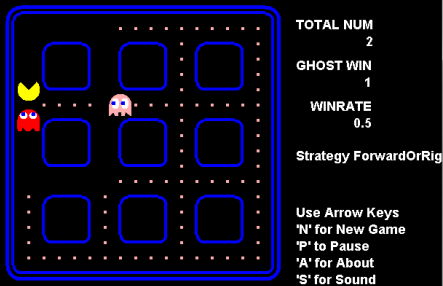
\includegraphics[width=0.5\textwidth]{ch3pacman}
	\caption{Zjednodušená verze Pac-Mana. Obrázek převzat z \cite{18Pac1}}
	\label{fig:ch3pacman}
\end{figure}

\subsection{Tvorba DDA pomocí MCTS}

Výkon umělé inteligence soupeřů založených na MCTS záleží na množství času, které MCTS poskytneme. Čím déle algoritmus běží, tím je pravděpodobnější inteligentnější chování duchů.

Postava Pac-Mana byla simulována hráčem, který měl nastaven několik pevně daných pravidel chování.

Pomocí opakovaných simulací s pevně daným simulačním časem získali závislost poměru vítězství (win-rate) na délce simulace. Několik získaných diskrétních hodnot proložili polynomem 4. stupně.

\begin{equation}
	y=-5,67*x^4+17,6*x^3-11,1*x^2-0,81*x+65,6
\end{equation}

V předchozí rovnici je x časem výpočtu MCTS v ms a y výsledné win-rate.
Běžný hráč chce vyhrávat přibližně v polovině případů. Vyřešením rovnice získáváme čas 105ms. Začínající hráč může upřednostnit častější vyhrávání, při win-rate 30\% (duchy) algoritmus potřebuje 28ms na výpočet.

\subsection{Využití neuronových sítí}
Další nevýhodou škálování AI pomocí změn simulačního času je horší využitelnost u real-time her, kde si nemůžeme dovolit věnovat stovky ms k výpočtu AI. Tento nedostatek lze odstranit využitím neuronové sítě místo MCTS.

Neuronovou síť se snažíme naučit chování odpovídající MCTS s daným simulačním časem. Při simulacích pomocí MCTS se při každém rozhodování duchů uložil stav hry, jako 23 proměnných a výsledné rozhodnutí o novém směru každého ducha.

Takto získaná data bylo použita pro učení neuronové sítě, která posléze nahradila původní algoritmus MCTS. Vstupními proměnnými byly např. pozice a směr hráče, pozice duchů a obsah sousedních dlaždic, vzdálenost mezi duchy a hráčem, čas simulace atd. Ve výstupní vrstvě bylo po 4 neuronech pro každého ducha, kde každý neuron představoval jeden zvolený směr.

Neuronové sítě odstranily časovou divergenci pro různé AI, ale naopak přinesly do systému jistou míru nepředvídatelnosti.
